\chapter{Mechanical Contact}\label{methodology-contact}

\section{Collision Detection}
  \subsection{Overview}
  This section is dedicated to collision detection and other relevant concepts. Starting with the general description of the process it identifies the main problem that occurs when dealing with collision detection. It also provides description of the various solutions to the problem, such as: utilizing spatial decomposition techniques and using parallel processing.
  \subsection{Description}
    Collision detection is essentially the process of identifying if two given objects are colliding. The term collision determination refers to the process of identifying the exact point of collision and potentially the interpenetration of the two objects. However, generally, collision detection includes the process of collision determination as well.

    In case of this particular project, we consider collision detection between polygonal meshes representing the main acting bodies during the childbirth process. The polygonal meshes consist of a number of (generally triangular) polygons arranged to represent an approximation of a given object. It is also worth mentioning that, this representation only gives the description of the surface of the object omitting the internal volumetric structure.


A na\"{\i}ve approach to collision detection involves testing each pair of triangles for intersections. The computational complexity of this process will be $O(n^2)$ \citep{gpuGems32}, which, in case of models with a high polygon count $n$, can yield reduced performance hence low frame rates. The most popular solution to this problem is spatial partitioning using Bounding Volume Hierarchies (BVH). This approach subdivides collision detection into two consequent phases. The first process, often called the broad-phase, involves pruning of the more distant (unlikely to collide) polygons from the list of all polygons to undergo the intersection tests, leading to reduced complexity $O(n~log~n)$ \citep{MPI}. After a small number of potentially colliding polygons is identified, the narrow-phase collision detection takes place. This phase involves pairwise intersection tests on the set of identified triangles. A more detailed description of the whole process is given in the following sections.

  \subsection{Broad Phase}
  As mentioned above, medical simulations deal with high polygonal meshes and require implementing a BVH. There are several types of BVH's, which differ in terms of bounding volume shapes and degrees. Here we will give descriptions for the different types of BVH's and provide justification for the option chosen to be implemented.

    \subsubsection{Bounding Volume}
    The term Bounding Volume (BV) refers to the simpler volume, which can be used to approximate the position and shape of a more complex triangular mesh. There are several options for a BV shape: sphere, axis-aligned bounding box (AABB), oriented bounding box (OBB), discrete orientation polytope (k-dop), line sweep sphere or convex hull \citep{BVs}. Figure \ref{BVs} illustrates the listed bounding volumes. A Bounding Volume Hierarchy (BVH) is a hierarchical collection of BV's, which can be represented as a tree.

          \begin{figure}
            \centering
              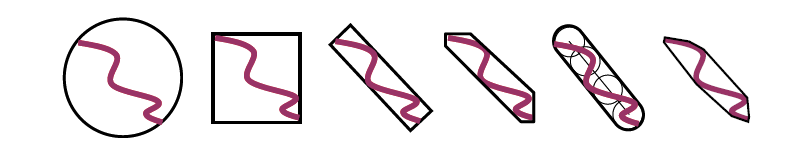
\includegraphics[width=120mm]{sections/methodology/images/contact/BVs.png}
            \caption[Different bounding volumes enclosing the same shape.]{\label{BVs} Different bounding volumes enclosing the same shape. From left to right: bounding sphere, AABB, OBB, k-DOP, line sweep sphere, convex hull from \citep{BVs}.}
          \end{figure}

    The bounding sphere has equal extents in all possible directions from its centre, which are equal to the radius of the sphere. AABB is represented by a box, which has three extents: width, length and height. The box is always oriented to match the axes of the world coordinate system. The difference between OBB and AABB is that OBB can have any arbitrary orientation. The k-dop's can have k number of vertices (in 2D) and represent a BV with arbitrary complexity, thus providing an adaptive solution \citep{realTimeColDet}. Convex hulls provide accurate approximations for the objects, which are always convex \citep{convexhulls}.

    Each of the BV shape options have advantages and disadvantages in terms of intersection testing and tightness of fitting. The bounding sphere and AABB allow simpler intersection tests, but suffer from poor fitting. OBB's, k-dop's and convex hulls provide tighter bounding, however require complex intersection tests. Figure \ref{BVs} demonstrates the difference in fitting for the different BV shapes.

    \subsubsection{Degrees of the Tree}
    Another aspect of the BVH is the maximum number of children that any given node in the tree can have. This number is often called the degree of the tree. There are several popular types of BVH's that are represented by trees with different degrees: binary tree, quadtree and octree. A binary tree has the degree of two allowing a maximum of two children for each node; four and eight children for the quadtree and octree respectively.

    In our simulation system we built two types of BVH collision detectors. The two differ in the degree of the tree that they represent. The Bitree and Octree

    \begin{figure}
    \begin{minipage}[t]{7cm}
    \begin{center}
    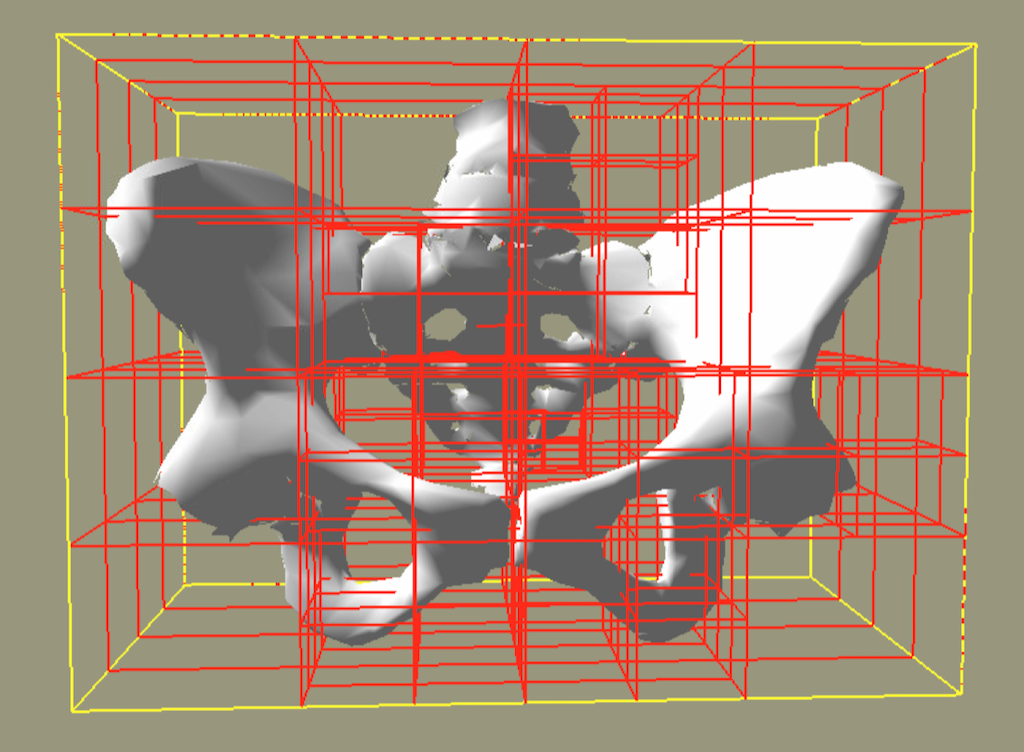
\includegraphics[width=70mm]{sections/methodology/images/contact/bvh-octree.png}
    \caption[A model of a pelvis with its BVH created using our Octree subdivision algorithm.]{\label{contact-octree} A model of a pelvis subdivided our Octree subdivision algorithm.}
    \end{center}
    \end{minipage}
    \hfill
    \begin{minipage}[t]{7cm}
    \begin{center}
    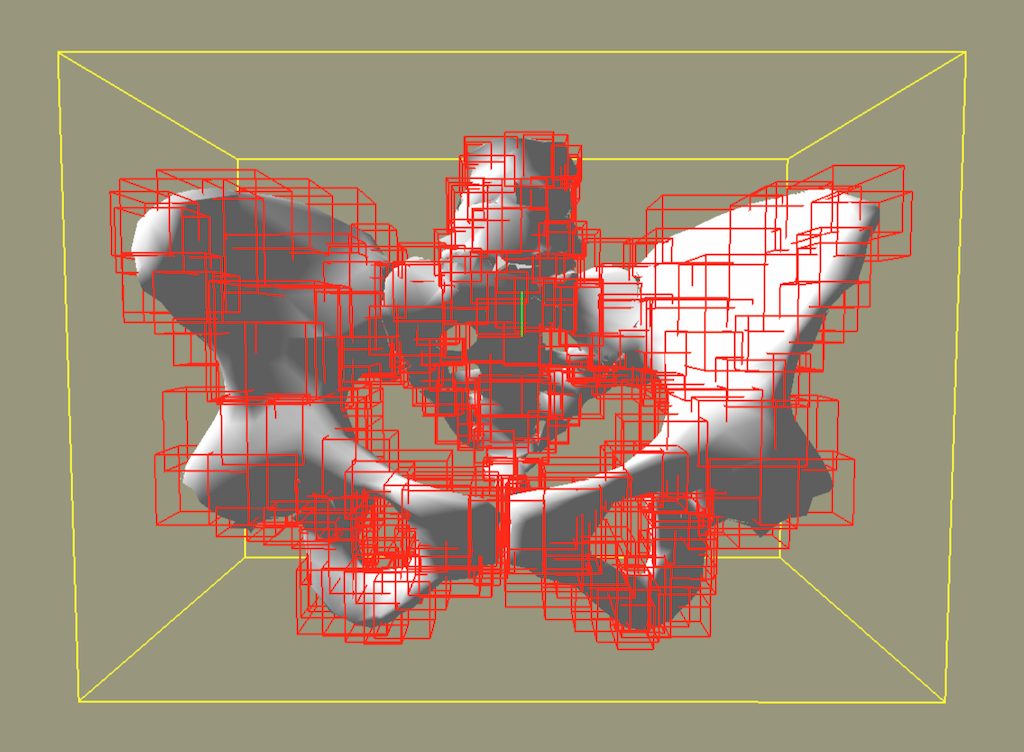
\includegraphics[width=70mm]{sections/methodology/images/contact/bvh-bitree.png}
    \caption[The same model subdivided using our Bitree algorithm.]{\label{contact-bitree} The same model subdivided using our Bitree algorithm.}
    \end{center}
    \end{minipage}
    \end{figure}

    \subsubsection{Intersection Detection}
    The main characteristic of a BVH is that the parent node encapsulates all of its children, therefore if a BV is disjoint with the parent it is also disjoint with all its descendants. This property can be used to prune a large number of polygons that cannot intersect. Thus the process of collision detection between two BVH's is performed by traversing both trees to identify intersecting leafs. The following pseudo code can be used for finding intersecting nodes of the two BVH's. The \emph{broad} phase ends when two intersecting leafs are found.


    \subsubsection{Analysis}
  \label{USINGOBBs}
    The AABB approach was implemented initially, as it is widely used in interactive graphical applications like games and simulations \citep{AABBUse}. This approach works well for the simulation where there are no rotations involved. The nature of the childbirth simulator requires the objects to be rotated in 3D space. As stated before AABB's are always aligned with the world coordinate system and when the bounded object is rotated they can fail to encapsulate the object properly and need to be rebuilt.

    Using OBB's allows arbitrary rotations of the objects, by changing their orientations. However, as already mentioned, using OBB's instead of AABB's requires more complex intersection tests. The AABB's intersection tests requires only a three axis test, whereas OBB's require 15 axis tests for the axes of each OBB and their cross products \citep{realTimeColDet}.

    The orientations of the tested OBB's are usually represented by matrices as suggested in \citep{realTimeColDet}. One way to perform the OBB intersection tests is by modifying the extent vectors of each of the boxes by their orientation matrix. However, one of the vector by matrix transformations can be avoided if the tests are performed locally to one of the OBB's. This can be achieved by calculating the transformation matrix that represents the first OBB in the coordinate frame of the second and performing the transformation only on the second. Figure \ref{localizationFig} illustrates the idea. In the cases when the BVH consists of many OBB's this can improve the performance. Equation \ref{localization} can be used to calculate the localization matrix.


                \begin{figure}
                \begin{minipage}[t]{6cm}
                \begin{center}
                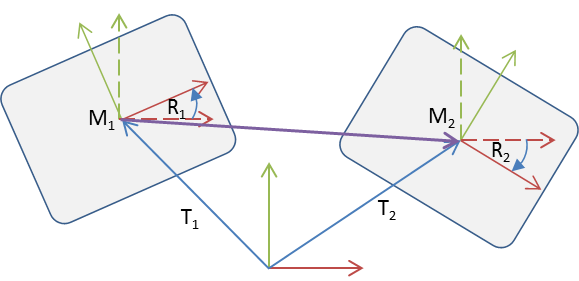
\includegraphics[width=65mm]{sections/methodology/images/contact/localizationOne.png}
                \caption[Global and local coordinate frames of OBB's.]{\label{localizationFig1} Global and local coordinate frames of OBB's are shown with dotted and solid arrows accordingly.}
                \end{center}
                \end{minipage}
                \hfill
                \begin{minipage}[t]{6cm}
                \begin{center}
                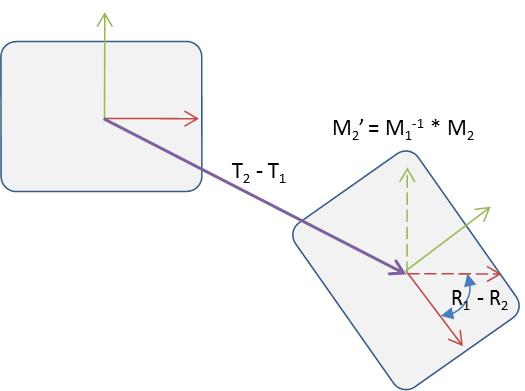
\includegraphics[width=65mm]{sections/methodology/images/contact/localizationTwo.png}
                \caption[Transforming coordinate frames.]{\label{localizationFig} Representing the right OBB in the coordinate frame of the left.}
                \end{center}
                \end{minipage}
                \end{figure}

\begin{equation}\label {localization}
M_{2}' = M_1^{-1}\cdot M_2,
\end{equation} where $M_2$ - \textit{from} matrix, $M_1$ - \emph{to} matrix, $M_2'$ - localization matrix from $M_2$ to $M_1$.


  \subsection{Narrow Phase}
  The \emph{narrow} phase of collision detection involves determining the exact intersections between polygons identified during the \emph{broad} phase. The generally accepted approach for testing polygon-polygon intersection uses the Separating Axis Theorem (SAT). The SAT states that, if two polygonal objects are not colliding, there exists an axis that separates the projections of the objects onto that axis. Thus, if an axis on which the projections of the objects do not overlap is found, the objects are not intersecting. The important point here is that the number of test axes is fixed and the number of required tests is calculated as in \ref{satnumberaxiseq}. For triangles the number of axes is 2 face normals and 9 edge vectors and their cross products.

  \begin{equation}\label{satnumberaxiseq}
  N_{t} = f_{1} + f_{2} + e_{1}\cdot e_{2},
  \end{equation}
  where $N_{t}$ - number of required tests, $f_{n}$ - number of faces of the $n$-th object, $e_{n}$ - number of edges in the $n$-th object.

  There are several implementations of the SAT for determining intersection between two triangles and the one presented in \citep{SAT} presents a suitable solution.


\section{Basic Mechanical Contact Model}

  \subsection{Basic Contact Model}

  The contact model used in our childbirth simulation system is described in terms of calculating the crucial physical values. The entities are: friction between the fetal head and the pelvis, forces and rotational moments arising from the contact. The Figure \ref{contact} describes the model in more detail.

  \begin{figure}
  \begin{center}
  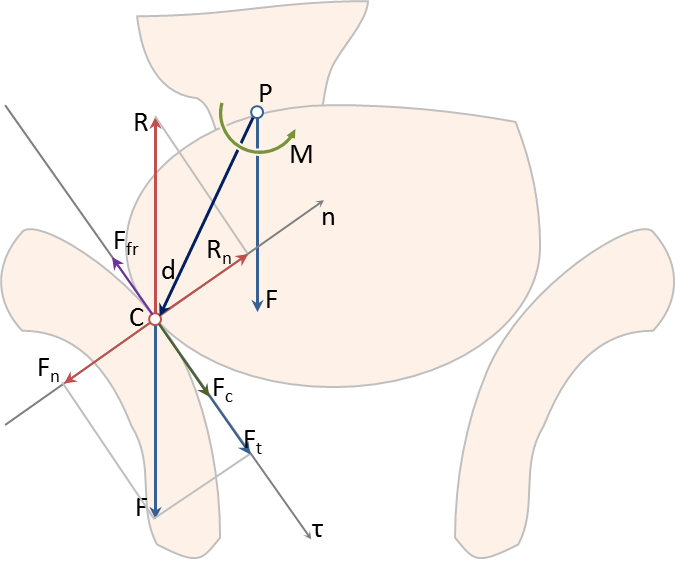
\includegraphics[width=100mm]{sections/methodology/images/basic/contact.png}
  \caption[A contact between two objects.]{\label{contact} A contact between two objects: \emph{P} -- pivot point, \emph{C} -- contact point,  \emph{F} –- external (uterine) force, \emph{R} –- reaction (contact) force, $F_\tau$ –- tangential component, $F_n$ –- normal component, \emph{n} -– contact normal, $\tau$ -– tangent plane, \emph{d} - radius vector, $F_{fr}$ -- friction force, $F_{c}$ -- contact force, $M$ -- the resulting rotation moment.}
  \end{center}
  \end{figure}


  \subsubsection{Friction}

    \begin{figure}
      \centering
        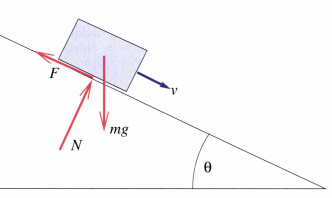
\includegraphics[width=60mm]{sections/methodology/images/basic/friction.png}
    \caption[Simple rigid body friction problem.]{\label{frictionFig} Simple rigid body friction problem: \emph{F} – friction force, \emph{N} – normal contact force, \emph{mg} - gravitational force, \emph{v} - velocity, $\theta$ - angle between the surface and horizontal plane}
    \end{figure}



    One of the most often used models for calculating friction between two rigid bodies in contact is Coulomb's law of friction \citep{coulomb00}. As illustrated on the Figure \ref{frictionFig}, the law states that the friction force is defined by the normal contact force \emph{N} times the coefficient of friction ( $\mu$ ). In case of a sliding contact, the friction force is exactly equal to $\mu$\emph{N} by magnitude. The direction is defined to be opposite to the tangential component of the acting force.

    The physical model to be used in the childbirth simulation will replace the gravitational force with the uterine contraction force. However, there is a need to specify a suitable friction coefficient for the head-pelvis contact. During the literature review no resources were found where the exact coefficients for this particular case are specified. The work by \citet{boneFrictionCoefficient} performed series of experiments and identified friction coefficients between a muscle and a bone. These values vary under different loads between $0.29$ and $0.36$. Considering that it is not the bare bones interacting, the friction coefficients of lubricated skin were examined. The works by \citet{skinFrictionInVivo} and \citet{realTimeSkinFriction} provide the coefficients, but the values vary widely according to the normal loads and the used lubricants. As it is difficult to choose a single value an average of $0.35$ was chosen as the starting option. The value can be changed during further experiments.


  \subsubsection{Rotational moments}
    In order to calculate rotational moments caused by collisions it is necessary first to identify a rotational pivot. For the rotational pivot of the fetal head the atlanto-occipital point (Fig \ref{basic-ao-point}) will be chosen. The rotational moment \emph{M} is found by calculating the cross product of the contact force $F_c$ vector and vector (\emph{d}), being the position vector from the rotational point to the point of contact. Equation \ref{calculateInitMoment} shows the relation:

    \begin{equation} \label{calculateInitMoment} \vec{M}=\vec{F_c}\times \vec{d} \end{equation}


    However, the contact force $F_c$ needs to be calculated first. The force is the resulting force acting on the fetal head during contact. It comprises of the normal, tangential and frictional components.

    The normal component is trivial to find by projecting the inverted external force onto the contact normal as in equation \ref{projectNormal}.

    \begin{equation}
    \label{projectNormal}
    \vec{F}_n = (\vec{F} \cdot \vec{n})\widehat{n}
    \end{equation}

    The tangential component $F_{\tau}$ of the reaction force is more ambiguous to find. It is known that the normal component is collinear with the normal and the tangential component will be inside the tangent plane as in Figure \ref{tangentFig}, but the plane contains potentially an infinite number of such vectors. However, considering the intersection of the tangent plane with the plane formed by the normal and the force \emph{F} it is possible to find the tangent vector. Thus, the direction of the tangential component is calculated from the contact normal and the external force \emph{F} using equations \ref{projectNormal},  \ref{findingTangent1} and \ref{findingTangent2}.

    \begin{figure}
    \begin{center}
    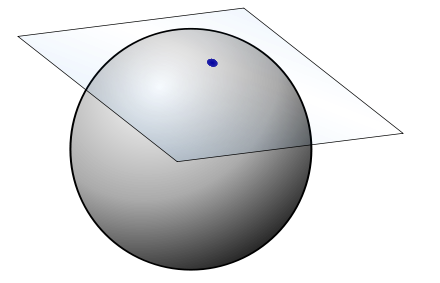
\includegraphics[width=65mm]{sections/methodology/images/basic/tangentspace.png}
    \caption[Tangent plane of a contact]{\label{tangentFig} Tangent plane of a contact}
    \end{center}
    \end{figure}

    \begin{equation}
    \label{findingTangent1}
    \vec{R}=-\vec{F} ~~ \wedge   ~~\vec{F_{\tau}}=\vec{F}-\vec{F_{n}}
    \end{equation}

    \begin{equation}
    \label{findingTangent2}
    \vec{F_{\tau}}=\vec{F}-(\vec{F} \cdot \vec{n})\vec n
    \end{equation}

    Thus, after identifying all the necessary forces for the contact the resulting contact force $F_c$ is defined as in equation \ref{findingFc}. Equation \ref {calculateInitMoment} can be worked out now. The rotation of the object is then calculated based on the combined rotational moments as seen in equation \ref{combineMoments}. It should be noted that each of the moments are calculated for each contact point separately.

    \begin{equation}
    \label{findingFc}
    F_c = F_{\tau} - F_{fr}
    \end{equation}

    \begin{equation}
    \label{combineMoments}
    M_{comb}=\sum_{i}^{n}M_{i}
    \end{equation}

\section{FE Based Mechanical Contact}
  \subsection{Principles}

    Explicit FEA techniques allow access to the forces resulting from the deformations of the finite element mesh. The forces are then used to update the deformations \textit{U} with an appropriate time integration technique. This feature results in a useful way to apply external force loads to the mesh, but also provides a way to extract force information at a particular contact point.

    The developed TLED framework can be represented as a pipeline as described in \ref{fea-algorithm}.  The first occurrence of the nodal forces in \ref{fea-algorithm-external-loads} is useful to apply external nodes. By the time the execution reaches the end of the time step, the buffer of forces is updated with the contributions from the deformed elements. The simulation module responsible for mechanical contact interaction can access the force data to perform contact calculations.

\section{Experiment}

  \subsection{Solid Sphere and Soft Cube Interactive Simulation}

    A simple scene was created as an initial testing setup for the TLED finite element simulation. As seen on Figure \ref{contact-sphere-cube} a solid sphere is moved into contact with a cube of a soft material.


    \begin{figure}
    \begin{center}
    \includegraphics[width=100mm]{sections/methodology/images/contact/sphere-cube.png}
    \caption[Solid sphere interacting with a soft cube simulated using GPU based TLED]{\label{contact-sphere-cube}}
    \end{center}
    \end{figure}
